\section{Projektplanl\ae{}gning}
Her gennemg\aa{}es essentielle projektplanl\ae{}gnings elementer. 

\subsection{Emnevalg}
I gruppen har der v\ae{}ret bred enighed om valg af emne. Retningen p\aa{} det emne var dog noget sv\ae{}rere at v\ae{}lge, men vi n\aa{}ede til enighed. 
Den endelige retning p\aa{} projektet blev f\o{}rst definitivt defineret meget sent i projektet.
Dette skyldtes at vi ikke fik lavet en grundig problemanalyse i starten af projektet.

For at lave en grundig problemanalyse kunne man i starten af P3 perioden indsamle og genneml�se mere materiale inden skriveprocesen igangs\ae{}ttes.
Dette ville kunne give et st\o{}rre indblik i emnet og hj�lpe med at finde en vinkel p� emnet fra starten.
%Dette kan forbedres til P3 ved at lave en grundig problemanalyse i starten af projekt perioden.

\begin{figure}[htbp]
\begin{center}
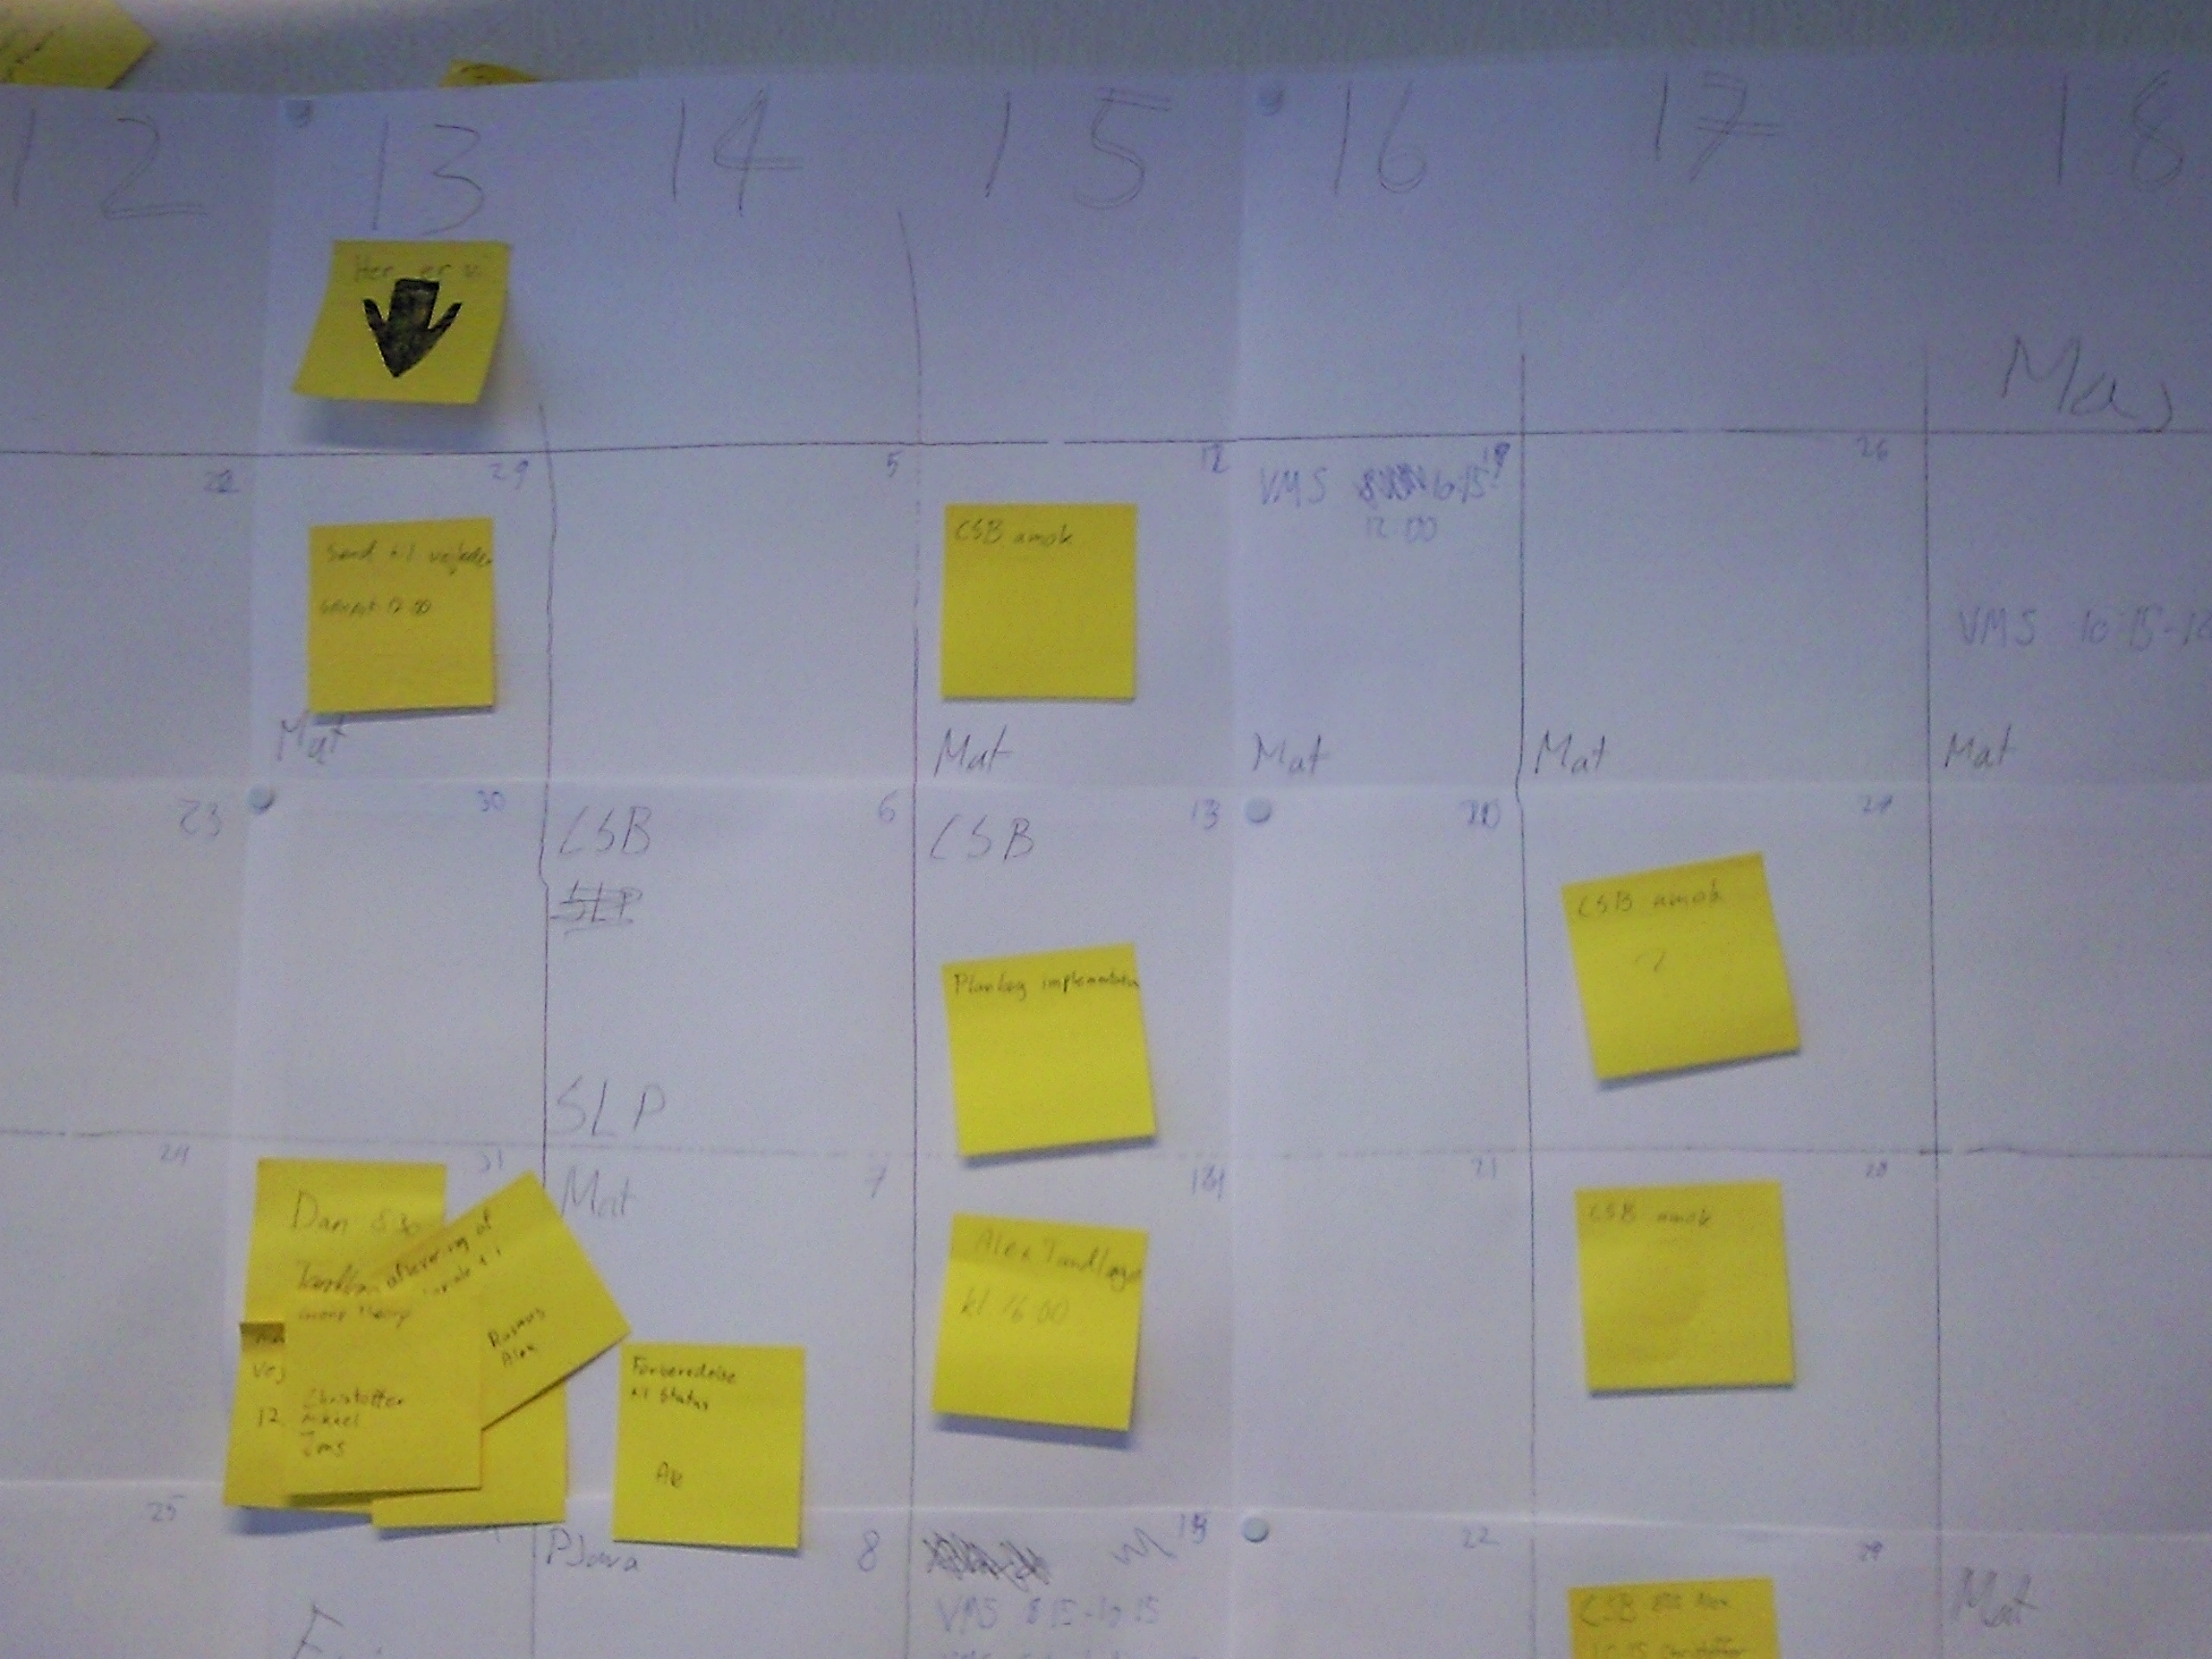
\includegraphics[width=\textwidth]{Billede0075.jpg}
\caption{Udsnit af vores v�gkalender}
\label{fig:vaeg}
\end{center}
\end{figure}


\subsection{Tidstyring}
Til at administrere projektets arbejdsgang og tidsplan har vi anvendt en v\ae{}gkalender (se figur \ref{fig:vaeg}). 

Kalenderen blev anvendt til at holde styr p\aa{} vores fastsatte deadlines. Hver opgave fik en deadline og en post-it, og blev p\aa{}sat den dato p\aa{} kalederen hvor opgaven havde deadline.
Kalenderen gav stor fleksibilitet idet post-its nemt kunne flyttes rundt hvis vi fandt ud af at en opgaves omfang var st�rre eller mindre end f�rst antaget.
%Dette gav en stor fleksibilitet hvis opgavens omfang var fejlvurderet og den p\aa{}kr\ae{}vede tid til l\o{}sningen var st\o{}rre end f\o{}rst antaget, kunne post-it flyttes til en ny dato. 
Kalenderen fungerede hensigtsm\ae{}sigt og gav et l\o{}bende overblik over hvor i projektet vi stod og hvordan vi er med tidsm\ae{}ssigt i forhold til deadlines. 
Dog med undtagelse af gennemretnings perioder. Her virkede kalenderen ikke hensigtsm\ae{}sigt og vi anvendte tavler til styring af hvilke rapportelementer der blev retter af hvem. 

Til senere projekter kan et lignende kalendersystem anvendes. Evt. en digitaliseret version da dette system optager meget v\ae{}g plads og da en digitaliseret version kan tilg\aa{}s hjemmefra. 

\subsection{Projektstyring}
I gruppen valgte vi en flad demokratisk styringsform. Denne styringsform fungerede fint; alle emner og problemer blev diskuteret l\o{}bende. En flad styringsform var mulig da vi stort set udelukkende arbejdede i grupperummet og derved altid havde mulighed for at diskutere problemstillinger med hverandre. 

Vi har i projektet haft nogle roller, herunder:
\begin{itemize}
\item Vejlederkontaktansvarlig
\item Kontorkontaktansvarlig
\item Trykkerikontaktansvarlig
\item Kasserer
\item Referent
\end{itemize}
Nogle af rollerne var ikke defineret og opstod mere eller mindre af sig selv, mens andre var fast defineret fra starten af projektperioden. Vejlederkontant, kasserer og referent var defineret. Referenten blev valgt til hver m\o{}de. 

Til P3 kunne der eksperimenteres med en defineret roterende lederrolle for at opn\aa{} nogle lederkompetencer til alle gruppens medlemmer. 






